
\chapter[Testes do Posicionador de Lente]{Testes do Posicionador de Lente}

 \textbf{\Large \center Caracterização de uma escala manométrica para testes de sensores de pressão}

Relatório de testes realizados para calibração de sensores de pressão utilizados para mensurar a força aplicada a um olho em um posicionador automático de lentes e de atuadores. 

\section[Fundamentos de Instrumentação Eletrônica]{Fundamentos de Instrumentação Eletrônica}

Instrumentação compreende atividades científicas, tecnológicas e industriais, relacionando fenômenos físicos, químicos e biológicos e suas percepções por humanos. Em todas as atividades humanas, a ideia de medição estabelece uma relação entre fenômenos e um grupo de símbolos, possibilitando uma representação confiável. O processo de medição é a base da pesquisa científica e industrial. Assim, a obtenção de dados experimentais trona-se essencial para a avaliação e aplicação de modelos teóricos desenvolvidos a partir do conhecimento físico-matemático.

Com base no conhecimento dos procedimentos e técnicas de obtenção de dados de fenômenos físicos, pode-se estabelecer alguns conceitos básicos de processos de experimentação.
\begin{itemize}
\item Processo de medição: processo de determinação de quantidades, graus ou capacidades comparando-as com unidades padrões estabelecidas em sistemas de unidades;
\item Instrumentação: tecnologia de verificação e medidas utilizadas em procedimentos científicos, industriais e médicos para verificação das quantidades e capacidades de fenômenos físicos;
\item Instrumento: dispositivo para determinar o valor ou magnitude de uma quantia ou variável.
\item Instrumento eletrônico: dispositivos de determinação de quantias e magnitudes que baseados nos conceitos de eletricidade.
\end{itemize}

Em um processo de aquisição de dados fundamentados em instrumentação eletrônica, tem-se por objetivo adquirir, condicionar e armazenar/mostrar os dados oriundos de fenômenos físicos. A Figura \ref{dados} apresenta um diagrama típico de um sistema de aquisição de dados.

\begin{figure}[H]
		\centering
			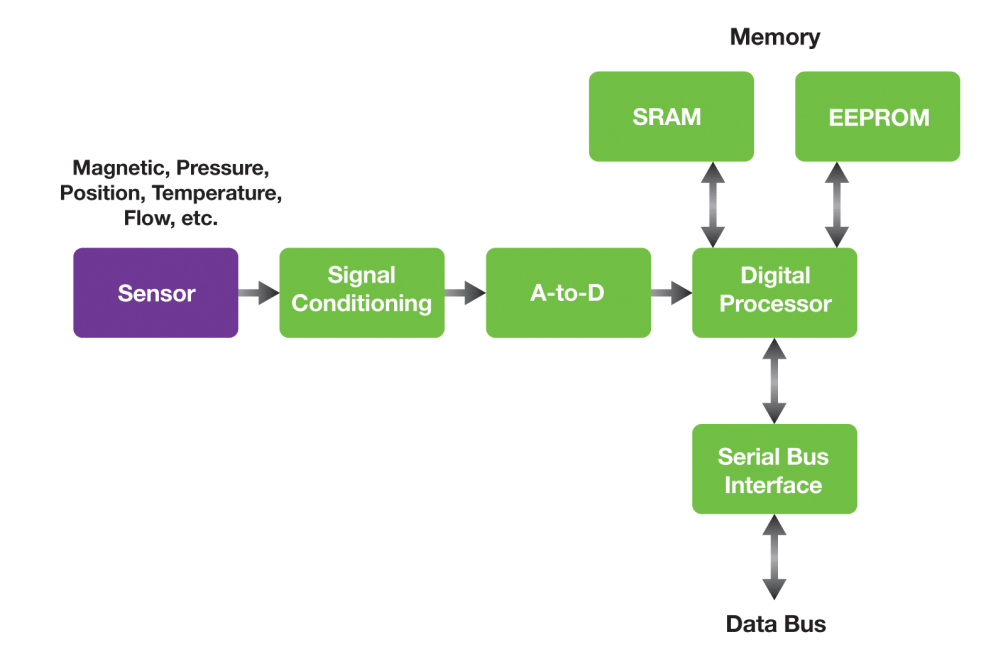
\includegraphics[scale=1.0]{figuras/diagramadados.png}
		\caption{Diagrama de um sistema de aquisição de dados}
		\label{dados}
\end{figure}

O foco de análise da equipe de instrumentação e testes para o posicionador de lentes enquanto sistemas de aquisição de dados são os sensores e transdutores utilizados para análise das condições ambientais para posteriores decisões do modulo de processamento. Para testar apropriadamente os sensores empregados no posicionador, têm-se como objeto de estudo as características dos sensores e transdutores que influem diretamente em seu modo de operação.

O desempenho de um instrumento pode ser analisado e caracterizado pelos seguintes conceitos classificados como características estáticas:
\begin{itemize}
\item Acurácia: grau de exatidão do processo de medição quando comparado aos valores desejados;
\item Resolução: a menor alteração no valor da variável ao qual o instrumento irá responder;
\item Precisão: medida da consistência ou repetibilidade do processo de medição;
\item Valor esperado: valor de cálculo ou o mais provável valor que se espera obter;
\item Erro: desvio entre valor verdadeiro e o esperado;
\item Sensibilidade: relação entre estímulos de entrada e a saída;
\item Faixa de atuação (Range): representa todos os níveis de amplitude do sinal de entrada nos quais se supõe que o transdutor opere, ou seja, intervalo de valores da grandeza em que pode ser usado o instrumento.
\end{itemize}

Os instrumentos para aquisição de dados de fenômenos físicos são classificados em sensores e transdutores. Sensores são instrumentos que podem detectar variáveis físicas, entregando como resposta uma saída mensurável que varia em relação a amplitude da variável física analisada. Transdutores são dispositivos que convertem um sinal de uma forma física para um sinal correspondente de outra forma física, fornecendo uma grandeza de saída que tem uma correlação específica com a grandeza de entrada. Podem ser classificados em função das aplicações em que são utilizados, a função que realizam, o princípio de funcionamento e/ou forma de energia que convertem. 

Uma das classificações mais adotadas na literatura diz respeito ao modo de operação destes instrumentos. Sensores/transdutores ativos são aqueles que geram um sinal de saída quando aplicada uma entrada sem necessitar de alimentação externa, enquanto que passivos requerem a entrada de energia para entregarem a resposta esperada. Os sensores de pressão utilizados no posicionador de lentes são de natureza passiva, necessitando de alimentação externa para seu correto funcionamento. O sensor de pressão utilizado é MPX5004DP. A Figura \ref{sensordiferencial} ilustra o sensor anteriormente mencionado.

\begin{figure}[H]
		\centering
			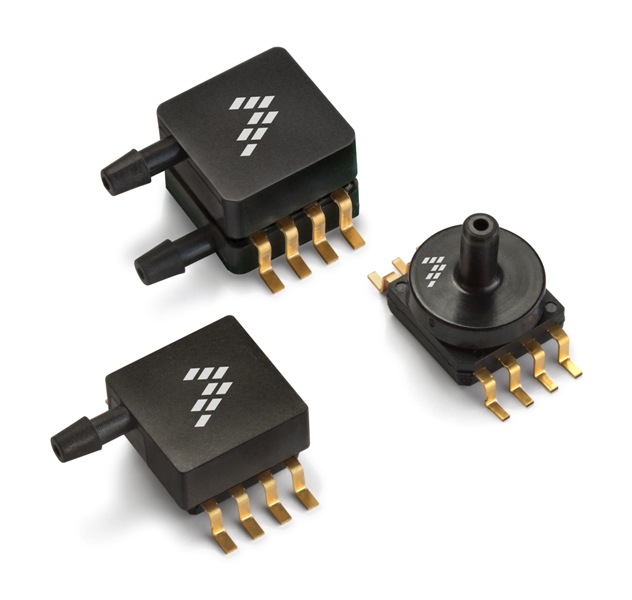
\includegraphics[scale=1.0]{figuras/sensordiferencial.png}
		\caption{Sensor diferencial de pressão mpx 5004DP}
		\label{sensordiferencial}
\end{figure}


\section[Experimentos Realizados]{Experimentos Realizados}

\subsection[Caracterização de uma escala manométrica para testes com sensores de pressão]{Caracterização de uma escala manométrica para testes com sensores de pressão}

Os sensores utilizados no projeto do posicionador de lente foram testados várias vezes, nas mesmas condições ambientais, utilizando os mesmos instrumentos de medição e pelos mesmos observadores. Afim de se obter uma análise posteriori satisfatória do sistema, realizaram-se testes de excitação dos sensores que compõem os módulos do posicionador, objetivando-se o levantamento da curva e melhor avaliação dos citados componentes. 

Para validar as pressões aplicadas aos sensores, fez-se uso de um manômetro de tubo em U como ilustrado nas figuras \ref{manometro} e \ref{manometro2}.

\begin{figure}[H]
		\centering
			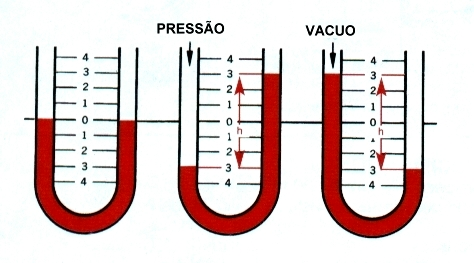
\includegraphics[scale=1.0]{figuras/manometro.png}
		\caption{Manômetro de tubo em U}
		\label{manometro}
\end{figure}

\begin{figure}[H]
		\centering
			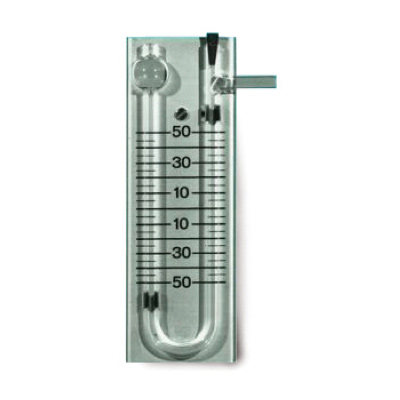
\includegraphics[scale=1.0]{figuras/manometro2.png}
		\caption{Manômetro de tubo em U real}
		\label{manometro2}
\end{figure}

O manômetro é um instrumento simples de medição indicado para baixos valores de pressão. É constituído por um tubo de material transparente, geralmente vidro, recurvado em forma de U e afixado sobre uma escala graduada. Seu princípio de funcionamento consiste na aplicação de pressão em um de seus ramos provocando o deslocamento do líquido presente em seu interior. Na condição de repouso (sem aplicação de pressão), há um equilíbrio de forças e a consequente nivelamento das colunas. O valor de pressão diferencial é dado pela diferença de altura entra as colunas do dispositivo, o valor de densidade do líquido utilizado e a gravidade. As unidades das constantes anteriormente mencionadas seguem os padrões do Sistema Internacional de Medidas para obtenção de resultados de mesma escala que os sensores utilizados.

Com o intuito de eliminar erros inerentes ao processo de medição, executaram-se três vezes os testes para um mesmo volume de ar. As aplicações de pressão foram feitas a partir do deslocamento do êmbolo de uma seringa. Foram utilizadas 20 graduações da seringa e para cada uma destas, o teste de verificação do valor de deslocamento da coluna de água foi realizado três vezes. A figura \ref{resultadosmanometro} apresenta os valores da altura em centímetros das colunas de água do manômetro. 

\begin{figure}[H]
		\centering
			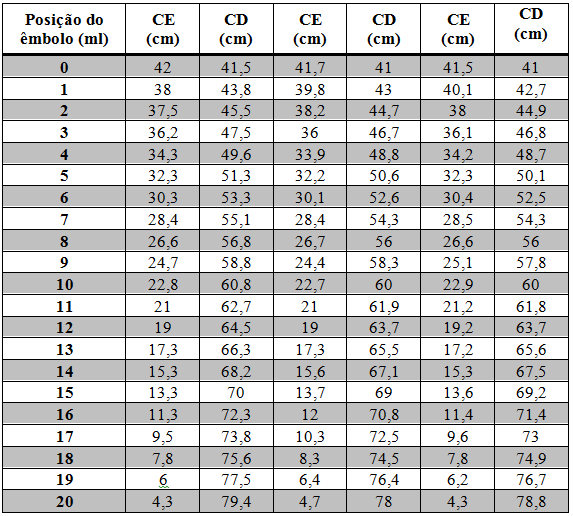
\includegraphics[scale=1.0]{figuras/resultadosmanometro.png}
		\caption{Resultados para testes de valores de pressão efetuados com um manômetro, onde CE, coluna a esquerda, CD, coluna a direita}
		\label{resultadosmanometro}
\end{figure}

Para analisar de maneira satisfatória os dados obtidos do experimento realizado com o manômetro, elaborou-se utilizando o software de simulação matemática MATLAB uma rotina para cálculo das medidas estatísticas dos dados obtidos. Calcula-se as medidas de tendência central, neste caso a média dos valores obtidos para uma dada graduação da seringa, e as de dispersão, neste caso o desvio padrão para um nível de graduação. 

Os valores de média obtidos a partir da rotina elaborada no MATLAB são apresentados na figura \ref{pressaomedia}. 

\begin{figure}[H]
		\centering
			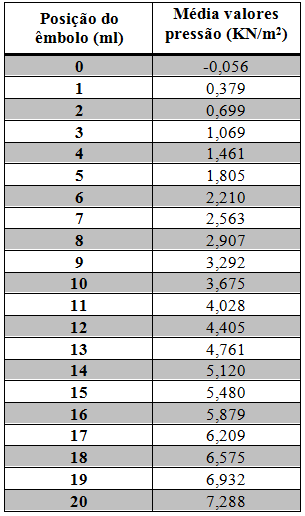
\includegraphics[scale=1.0]{figuras/pressaomedia.png}
		\caption{Valores médios de pressão para cada graduação de uma seringa}
		\label{pressaomedia}
\end{figure}

Os valores de pressão médios mostrados na tabela acima são dados em N/m2, unidade de pressão no S.I., Sistema Internacional de Unidades. A partir dos valores de pressão cálculos para cada graduação da seringa, construíram-se os gráficos para análise da variação de pressão diferencial a partir de um aumento gradativo de pressões aplicadas ao manômetro. Os gráficos apresentados na figura \ref{pressaoseringa} são resultantes de uma plotagem dos valores de graduação da seringa pelos valores de pressão. Os valores utilizados para a construção dos gráficos estão presentes na figura \ref{resultadosmanometro} previamente apresentada.

\begin{figure}[H]
		\centering
			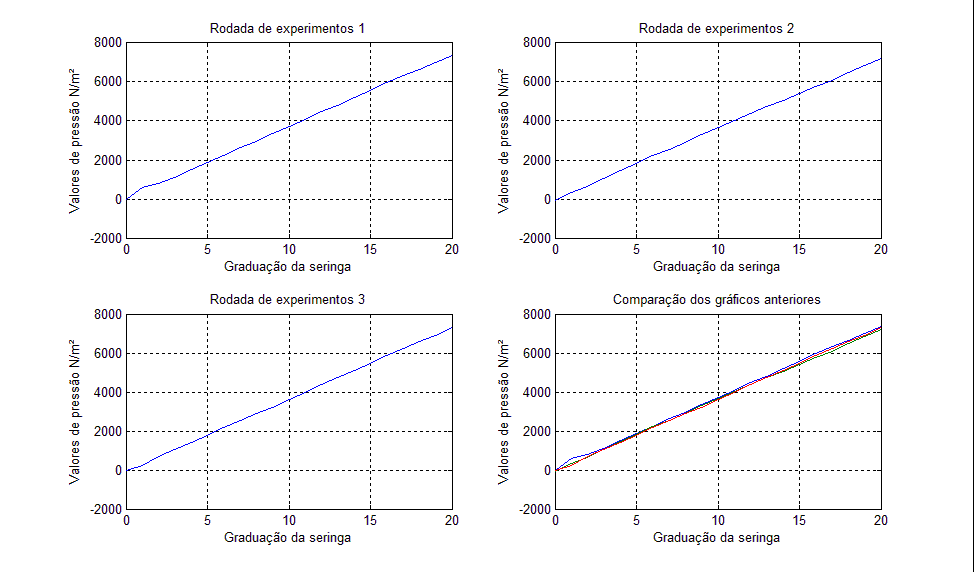
\includegraphics[scale=1.0, angle=90]{figuras/pressaoseringa.png}
		\caption{Gráficos de pressão para graduações da seringa}
		\label{pressaoseringa}
\end{figure}

A Figura \ref{mediapressaoseringa} apresenta o gráfico para a média dos valores de pressão por graduações da seringa.

\begin{figure}[H]
		\centering
			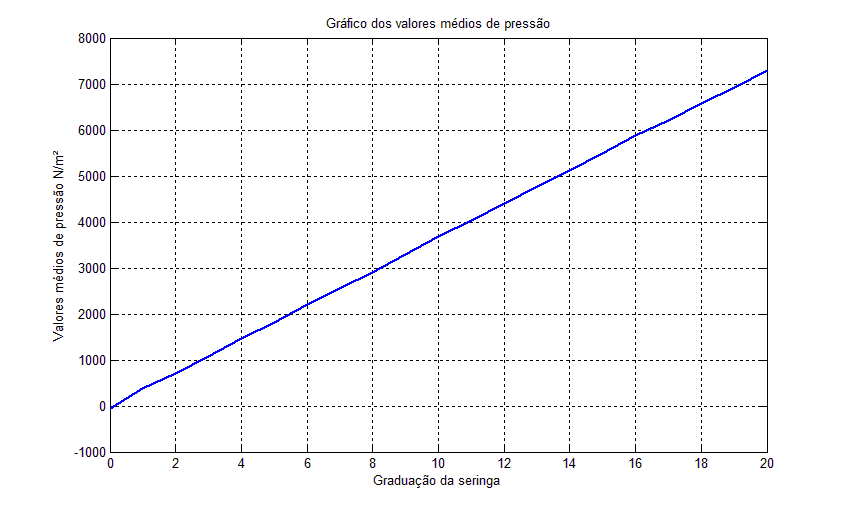
\includegraphics[scale=0.8]{figuras/mediapressaoseringa.png}
		\caption{Média dos valores de pressão para cada graduação da seringa}
		\label{mediapressaoseringa}
\end{figure}

As equações estimadas a partir dos valores experimentais resultantes do teste com o manômetro foram obtidas fazendo-se uso do método dos mínimos quadrados. Para cada rodada de teste, encontrou-se uma equação para caracterização do processo de variação da pressão diferencial decorrente do deslocamento do êmbolo da seringa. As equações são resultados de uma rotina escrita para determinação das equações estimadas considerando a graduação da seringa a variável independente e o valor de pressão diferencial a variável dependente. Os valores dos coeficientes das equações dos testes realizados são apresentados na figura \ref{equacoesmanometro}. As equações são de 1º grau e são escritas na forma y=b1*x+b0.

\begin{figure}[H]
		\centering
			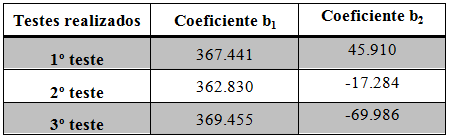
\includegraphics[scale=1.0]{figuras/equacoesmanometro.png}
		\caption{Coeficientes das equações estimadas para testes realizados com manômetro}
		\label{equacoesmanometro}
\end{figure}

A análise da dispersão dos dados coletados a partir do experimento baseia-se nos valores de desvio padrão calculados para cada graduação da seringa. A Figura \ref{desviopressao} apresenta os valores de desvio padrão para os dados resultantes dos testes e a figura \ref{graficodesvio} apresenta plotagem dos valores de dispersão.

\begin{figure}[H]
		\centering
			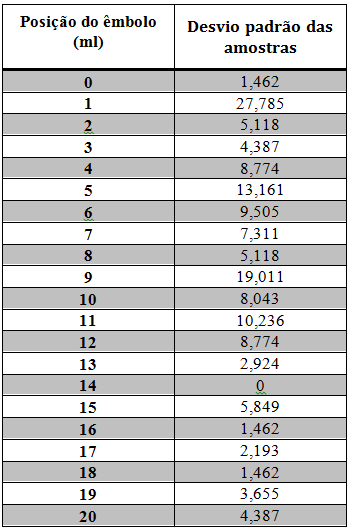
\includegraphics[scale=1.0]{figuras/desviopressao.png}
		\caption{Valores de desvio padrão para pressões}
		\label{desviopressao}
\end{figure}

\begin{figure}[H]
		\centering
			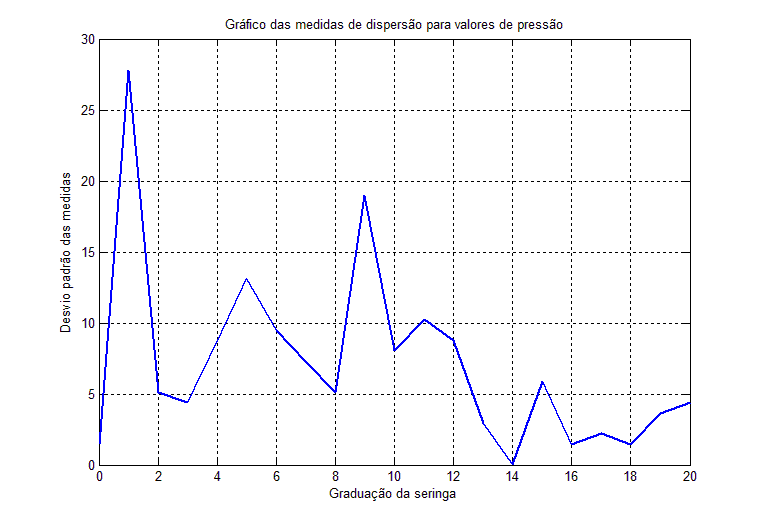
\includegraphics[scale=0.8]{figuras/graficodesvio.png}
		\caption{Gráfico de dispersão para valores de pressão}
		\label{graficodesvio}
\end{figure}

Baseando-se nos valores de dispersão encontrados, analisa-se a homogeneidade dos dados obtidos experimentalmente. O desvio padrão de um determinado grupo amostral mede o nível de variação em torno de uma dada média. Se a proximidade entre os dados analisados, o desvio padrão será pequeno, e consequentemente os dados serão homogêneos. Observando-se os valores de desvio padrão para cada graduação da seringa, nota-se que os valores são baixos, indicando baixa variabilidade das medidas realizadas conferindo fiabilidade ao processo de experimentação. A homogeneidade dos dados coletados é ainda confirmada por valores de coeficiente de variação. Trata-se de uma medida de dispersão relativa resultante da divisão dos valores de desvio padrão e a média amostral. Esta medida é definida como a razão entre desvio padrão e a média. Considera-se o coeficiente de variação baixo (indicando um conjunto de dados razoavelmente homogêneo) para valores inferiores a 20\%. A Figura \ref{graficocoeficientes} apresenta os valores de coeficiente de variação para cada graduação da seringa.

\begin{figure}[H]
		\centering
			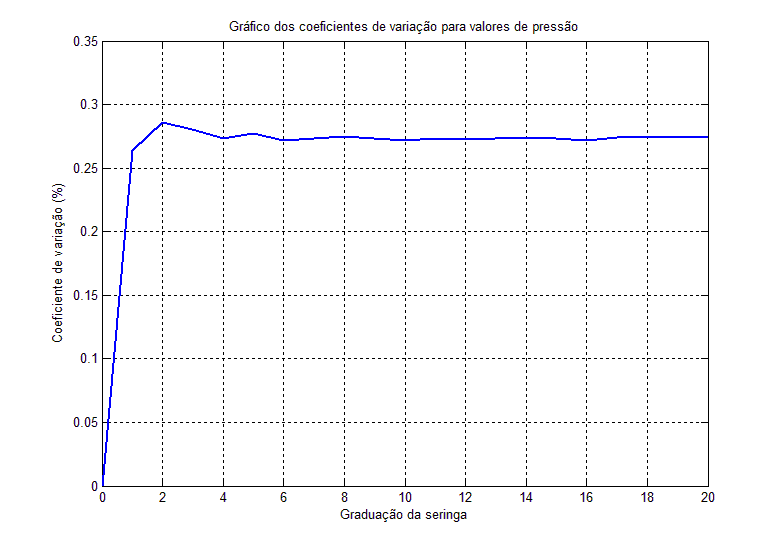
\includegraphics[scale=0.8]{figuras/graficocoeficientes.png}
		\caption{Coeficientes de variação para valores de pressão}
		\label{graficocoeficientes}
\end{figure}

Verifica-se com base no gráfico apresentado previamente que os valores de variação para os valores de pressão calculado a partir das amostras experimentais são inferiores ao limiar de homogeneidade estabelecido. 

\subsection[Teste do sensor de pressão MPX 5004DP]{Teste do sensor de pressão MPX 5004DP}

A série de transdutores piezo resistivos MPxx 5004 foi projetada para uma vasta gama de aplicações, particularmente as embarcadas onde há a utilização de micro controladores ou microprocessadores com entradas analógicas e digitais. Este dispositivo entrega como saída um sinal analógico proporcional a pressão aplicada. A figura \ref{sensor5004} apresenta as principais características deste sensor.

\begin{figure}[H]
		\centering
			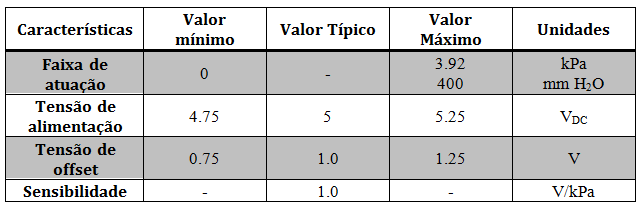
\includegraphics[scale=1.0]{figuras/sensor5004.png}
		\caption{Características do sensor de pressão MPX 5004}
		\label{sensor5004}
\end{figure}

As informações de acerca dos valores de pressão aplicados a partir de uma seringa serão utilizadas para validar as informações apresentadas na tabela acima. O comportamento esperado deste dispositivo é apresentado na figura \ref{respostasensor5004}. Nota-se que a resposta deste sensor é linear e diretamente proporcional as tensões de entrada aplicadas.

\begin{figure}[H]
		\centering
			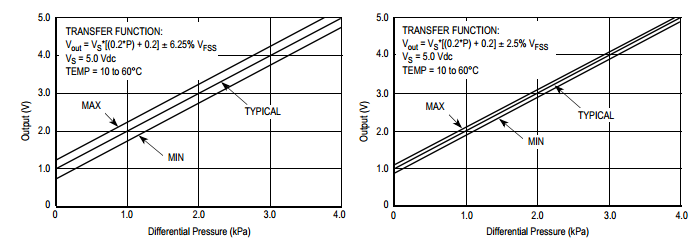
\includegraphics[scale=0.8]{figuras/respostasensor5004.png}
		\caption{Resposta esperada para o sensor de pressão MPX 5004}
		\label{respostasensor5004}
\end{figure}

A falta de uma estrutura de simulação apropriada para o olho humano inviabilizou o levantamento de mais dados acerca deste sensor quando conectado a ventosa de posicionamento da lente. No entanto, testaram-se os valores de pressão aplicados ao olho em duas situações distintas. A figura \ref{pressaoolho} apresenta os valores de tensão resultantes de uma simulação de acoplamento de lente a um olho humano. A Figura \ref{pressaoolho2} apresenta o teste realizado.

\begin{figure}[H]
		\centering
			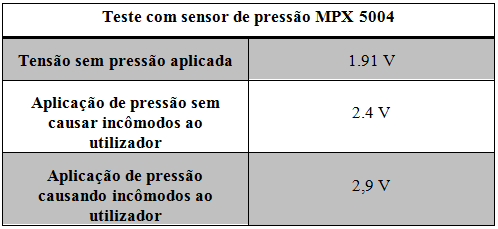
\includegraphics[scale=1.0]{figuras/pressaoolho.png}
		\caption{Teste de verificação dos valores de pressão para acoplamento de uma lente ao olho humano}
		\label{pressaoolho}
\end{figure}


\begin{figure}[H]
		\centering
			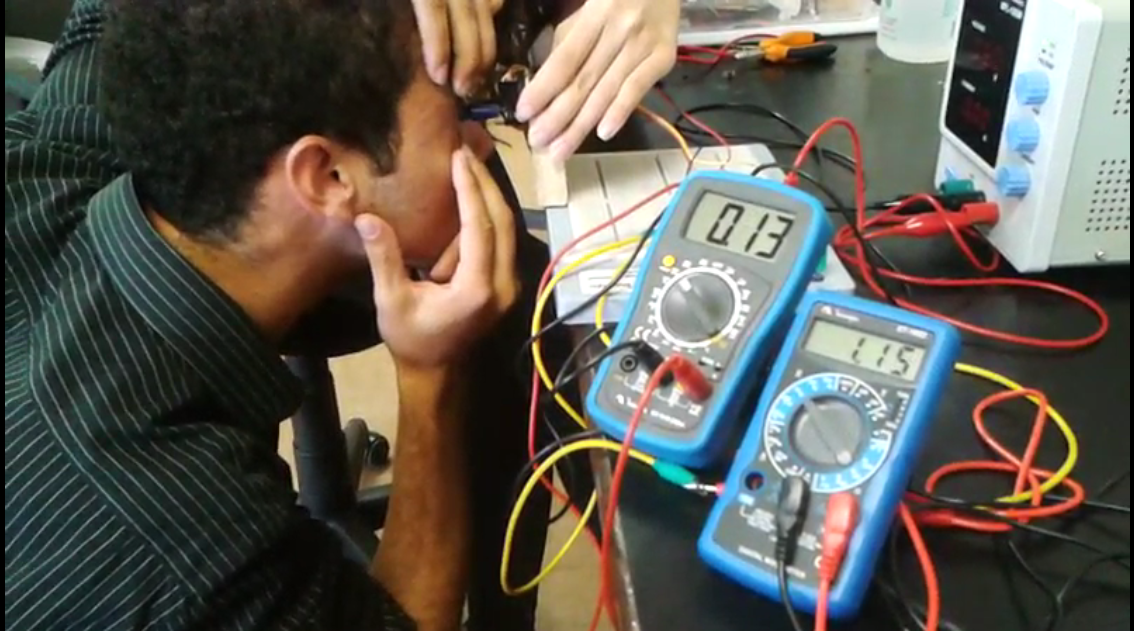
\includegraphics[scale=0.5]{figuras/pressaoolho2.png}
		\caption{Teste de acoplamento de uma lente ao olho humano}
		\label{pressaoolho2}
\end{figure}

\section[Conclusão dos Testes e Trabalhos Futuros]{Conclusão dos Testes e Trabalhos Futuros}

Conclui-se que o sensor escolhido para verificação de diferenças de pressão no interior da ventosa de acoplamento da lente foi escolhido corretamente, pois o simples contato entre a estrutura de acoplamento e o olho provoca variações na resposta do sensor. Os valores obtidos a partir do deslocamento de um serão utilizados para validação comportamental dos sensores de verificação dos limites de aplicação de pressão aos olhos.  A rotina escrita no software MATLAB para validação dos dados obtidos experimentalmente pode ser encontrada em Apêndices.